\documentclass[conference]{IEEEtran}
\IEEEoverridecommandlockouts
% The preceding line is only needed to identify funding in the first footnote. If that is unneeded, please comment it out.
\usepackage{ctex}
\usepackage{cite}
\usepackage{amsmath,amssymb,amsfonts}
\usepackage{algorithmic}
\usepackage{graphicx}
\usepackage{subfigure} %子图
\usepackage{textcomp}
\usepackage{xcolor}
\def\BibTeX{{\rm B\kern-.05em{\sc i\kern-.025em b}\kern-.08em
    T\kern-.1667em\lower.7ex\hbox{E}\kern-.125emX}}
\begin{document}


% \title{文章标题}

% \author{
% \IEEEauthorblockN{张三}
% \and
% \IEEEauthorblockN{李四}
% }

% \maketitle

\input{title.tex}

\begin{abstract}
  本项目是基于Unity的多人球类物理游戏,用Socket实现了联网对战,而没有使用内置或第三方的联网组件。玩家会依照规则分配到不同的队伍,灵活运用操作、技能与战术来进球得分。本项目做到了完备的游戏性、可靠的联网技术、美观及时的反馈三者有机统一,服务端与客户端统一为一个项目,在游戏程序中依仗用户操作和代码逻辑上的不同加以切换。项目中各部分各司其职,耦合度较低,且互相调用比较方便,为未来的开发、调试、增量都奠定了基础。
\end{abstract}


\section{引言}

本项目旨在解决Unity多人在线对战游戏开发的问题,联机系统为C/S模式,使用Socket技术独立开发。该游戏是一个基于物理的足球游戏,打开游戏并设定好端口号后即开启了服务端,其他人则只需输入专用服务器的IP地址和端口号便可加入游戏,即使是中途加入当前场上的状态也会同步过来;每位连接到服务器的玩家都会在一定规则下被分配到队伍,将球踢入其他队伍球门会加分,踢入自己队伍球门会扣分;玩家在游戏中有着丰富多样的策略,可以通过身体来带球,可以用四个角上的能量棒去“踢”球,还可以通过旋转能量棒改变球的走向,甚至借助蓄力来发动必杀技,一转局势;因为完全基于物理,玩家的移动等操作皆是通过施加力来实现的,不同物体的物理材质也有差异,如运用得当,可完成多次反弹进门等高难度操作;小地图、碰撞效果、蓄力显示等将给予玩家非常直观的反馈。

“独乐乐不如众乐乐”,多人游戏与单人游戏的快乐程度是在不同层次上的,不管是棋牌类的斗地主、麻将,还是竞技类的足球、篮球,亦或是流行的电子游戏《魔兽争霸》《英雄联盟》都为玩家们带来了单人时无法获得的快乐,许多人还会去观看其他人直播游玩多人游戏,从中获得欢愉。多人游戏也极大拓宽了一个游戏的丰富度,一个规则设置和维护得当的游戏,玩家可以游玩数年也不会感到厌倦。从开发的角度上,将一款游戏做成联机游戏的难度也与纯本地游戏是不可同日而语的,从建立连接、收发数据包到同步状态,还要考虑延迟、反作弊等各种复杂问题,Unity本身也没有内置合适的联网组件,这些对开发者来说都是一种考验。

我们在开题之初便对常用的Unity联网游戏实现方式进行了调研。首先,Unity内置的Unity Networking(UNet)已经被官方宣布为过时,并将在近两年彻底停止维护,从Unity中移除\cite{UNet过时};官方用于取代UNet的新联网组件——基于ECS架构的Unity NetCode,最新版本刚发布到 0.2.0,只是预览测试用的版本,无法正式投入实际开发;对于第三方的解决方案,Mirror算是基于UNet的改进版,但每个连接仅支持一个客户端;SmartFoxServer知名度低,国内外的文档都比较少;Photon为Client/Client的通信模式,并非我们需要的Client/Server模式\cite{优缺点比较},ET框架是一个组件系统,和我们熟悉的面向对象差异较大。综合考虑各个因素,小组成员决定通过较为底层的Socket直接开发我们希望实现的网络联机系统,相关代码完全透明,参考微软提供的.NET文档,有着高度的自定义性,也不用担心因第三方封装带来的未知bug。

我们从最基础的连接和收发包开始,先建立一个控制台的服务器和Unity中的客户端,接下来将服务器迁移到Unity中,随后再将二者合到一个项目中,共用场景。与此同时,本地也有一个测试场景,用来完成上线前的调试工作。网络部分,我们专注于场景中物体的创建、销毁、同步……玩家角色作为游戏中最重要的部分之一,从基础的移动逐渐丰富到能蓄力、能施展必杀技,有些效果的实现可能会对联网部分提出新的要求,此时便会一边开发网络部分,一边在本地开发效果部分。最后,还有一些用来增加游戏表现力的后期处理和辅助开发的实用代码。


\section{相关工作}
\subsection{Unity}
Unity是一个跨平台的游戏引擎,可用于创建三维、二维、VR、AR游戏,有着可视化编辑、操作简单、文档全面等优点,易于开发学习,深受大众的喜爱。《城市:天际线》《奥日与黑暗森林》《茶杯头》《人类一败涂地》等知名游戏皆是用Unity开发的。

\subsection{C\# Socket}
套接字是支持TCP/IP协议的网络通信的基本操作单元。可以将套接字看作不同主机间的进程进行双向通信的端点,它构成了单个主机内及整个网络间的编程界面。套接字存在于通信域中,各种进程使用这个相同的域用Internet协议来进行相互之间的通信。\cite{Unity3D网络游戏实战}

\begin{figure}[htbp]
    \centerline{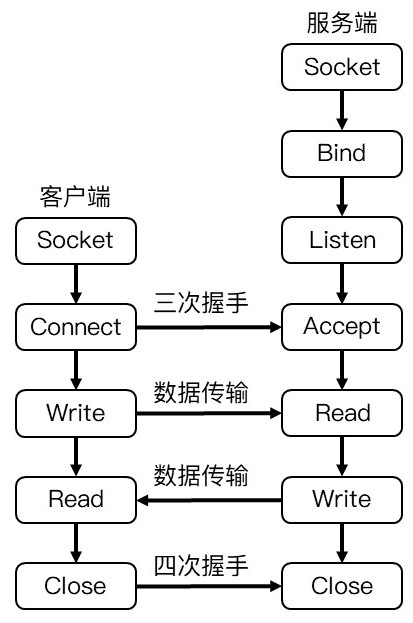
\includegraphics[width=.22\textwidth]{images/Socket通信的基本流程.jpg}}
    \caption{Socket通信的基本流程}
    \label{fig:socket}
\end{figure}


\subsection{Addressable Asset System}
Addressable Asset System提供了一种按地址加载Assets的简单方式,相比Resources和AssetBundle更加方便与灵活,能够进行自动化仓储管理和内存管理,只需要一个地址便可以从任意地方加载,默认的所有操作都是异步操作,可以添加事件监听。无需开发者自行收集与管理资源的依赖关系,且提供可视化界面,极其强大。

\subsection{Post Processing}
Post Processing是一个后期效果增强组件,可以在较少的时间内实现辉光、色彩分离、胶片颗粒、景深、运动模糊、镜头畸变、色彩调整等各种常用特效的效果,为整个游戏增光添彩,也减少了自己编写shader的困难。


\section{实践过程}

\subsection{Socket通信}
本次实践使用Socket技术完成服务端(Server)与客户端(Client)间的网络通信。因为游戏基于Unity,故底层使用了.Net框架System.Net(特别是System.Net.Socket)命名空间下的内容。与Socket通信相关的程序架构,借鉴了网络教程\cite{myCite:Tom},并在其基础上加以改进,使之更能满足开发和游戏运行时的需求。

为了方便复用代码逻辑及Unity资源,本次实践中将服务端与客户端置于同一项目,共享部分资源(例如一些游戏场景、Prefab、代码逻辑等)。最终构建出的程序可由用户手动选择充当服务端或客户端。

\begin{figure}[h!]  
	\setlength{\abovecaptionskip}{.2cm}   %调整图片标题与图距离
	\setlength{\belowcaptionskip}{0cm}   %调整图片标题与下文距离
    \centering  %图片对齐方式
    \subfigure[成为客户端] {
		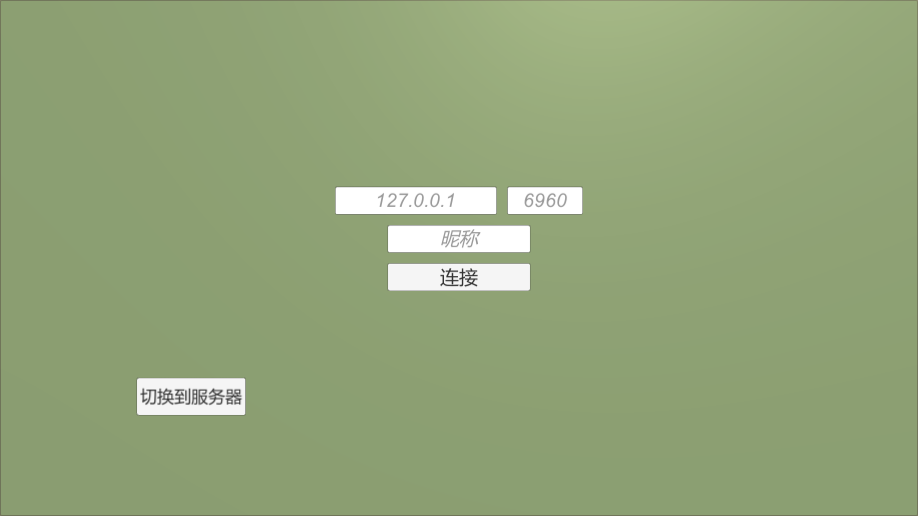
\includegraphics[width=0.45\textwidth]{images/beClient.png} 
    }
    \subfigure[成为服务端] {
		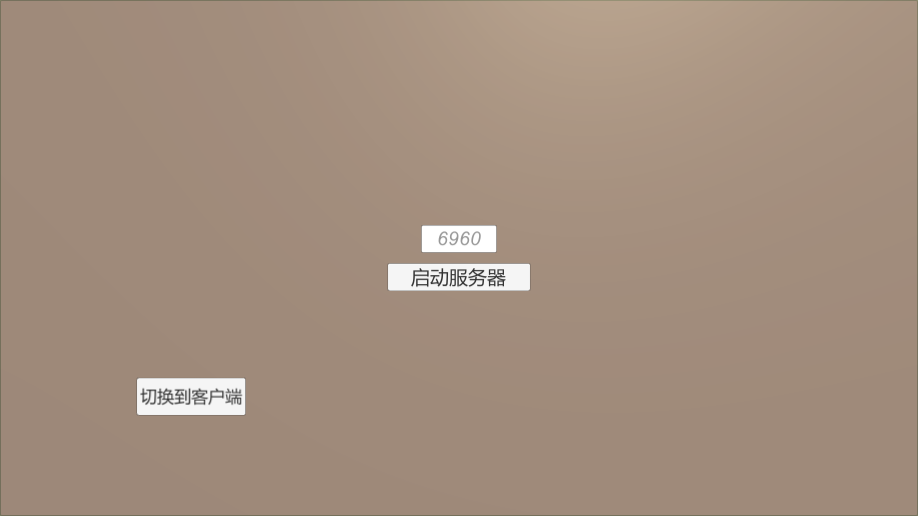
\includegraphics[width=0.45\textwidth]{images/beServer.png} 
    }
    \caption{选择成为客户端或服务端}
    \label{fig:beCS}
\end{figure}

\subsubsection{连接与断开}
\quad 

本项目在服务端同客户端通信的过程中,同时用到了TCP与UDP两种传输协议。服务端开启后,会非阻塞地监听其端口上的TCP连接请求和UDP报文;客户端向指定套接字连接的过程中,会先尝试同服务端建立TCP连接,通过TCP连接简单交换信息(如客户端ID和玩家昵称等)后再向服务端发送UDP报文,让服务端对客户端信息形成记录,为之后进行UDP通信做准备。

本项目中的所有代码逻辑均处于BallScripts命名空间下,并根据性质进一步细分。服务端逻辑在BallScripts.Servers命名空间;客户端逻辑在BallScripts.Clients命名空间。两命名空间中均包含Client类,内含内部类TCP、UDP,负责处理一个客户端的TCP、UDP相关逻辑。服务端还存在Server类,统筹多个Client对象;而客户端的Client为单例类,管理自身的连接及通信。服务端存在多个Client对象,意味着服务端同每个客户端都保持独立的TCP连接。但对于UDP,服务端使用统一的逻辑发送、接收数据,并根据Client对象中记录的客户端ID及套接字端点来确定要交由哪个Client对象做具体处理。

无论是服务端还是客户端,都存在主动断开连接的代码逻辑,即服务端可以主动断开同任意客户端的连接,客户端也可以主动断开同服务端的连接。一方断开时,另一方稍后也会自行关闭连接。

\subsubsection{数据包}
\quad

服务端、客户端间传输的内容,本质上是一些字节序列,虽然便于传输,却不方便理解与处理。为此,引入BallScripts.Utils命名空间下的Packet类,作为服务端和客户端共同的一种约定,将字节序列包装成使用起来更方便的数据包。

一个Packet对象让代码能够写入或读取一些常见的数据类型(如int、float、string、Vector3等),从而灵活地组装或使用字节序列。此外,在构建字节序列并发送的过程中,数据包能够自动为字节序列补充长度信息;如果数据包从客户端发送,则还会包含其客户端ID。

程序执行到任何逻辑,但凡需要网络通信,便要构建并发送数据包。这些数据包携带的数据往往不同,需要一种标识来加以区分,让接收方知道这些数据包分别代表何种逻辑。这种标识可以通过枚举实现,来自服务端的数据包使用ServerPackets枚举;来自客户端的数据包使用ClientPackets枚举。标识会以整数的形式附在数据包内。

\subsubsection{发送、接收}
\quad

服务端和客户端,各提供一组专门的方法来发送、接收不同标识的数据包。

创建并发送数据包的逻辑,在服务端位于ServerSend类,在客户端位于ClientSend类。两个类中包含若干公有(public)、静态(static)方法,一种持有特定标识的数据包至少会对应其中一个。根据各方法中使用的不同逻辑,数据包会被写入不同的标识、数据,并通过TCP或UDP发送(一般需要可靠传输的重要信息通过TCP发送,发送频率较高且相对不重要的信息,如物体位置等,通过UDP发送)。在服务端,有时还允许指定数据包的发送对象,可以是所有已连接的客户端或某些特定客户端。

接收并处理数据包的逻辑,在服务端位于ServerHandle类,在客户端位于ClientHandle类。类中同样有若干公有、静态方法,这些方法的名称与数据包持有的各种标识相对应。例如,在客户端,ClientHandle中的各方法,名称同ServerPackets中的枚举项对应。这些方法的参数列表也被统一规定,在程序初始化时以ServerPackets项为键、存储着ClientHandle方法的委托为值,纳入字典中统一管理。这样程序收到数据包后,根据其标识即可在字典中找到相应的处理逻辑,进而通过得到的逻辑处理数据包。大致相似的布置和流程在服务端中也存在。

为了不让接收数据包的逻辑同各种游戏逻辑大量耦合,又分别设置了ServerLogic类与ClientLogic类,用于放置一些真正和游戏逻辑有关的方法,部分方法传入从数据包中得到的数据,运用它们更新场景信息、执行游戏逻辑乃至发送新的数据包。

\subsection{场景物体}
为了标识并管理场景中的各种物体,我们在MonoBehaviour的基础上定义了BaseStageObject类。任何出现在游戏场景中的物体都会拥有BaseStageObject或其子类作为组件,其中记录了该物体存在于场景中所必要的一些信息。
\subsubsection{管理、同步}
\quad

BaseStageObject中最重要的,便是物体的种类(category)和编号(id)信息。种类是人为定义的枚举值,有6种可能——Player、Ball、Goal、Dynamic、Static、Other;而编号则是整数,一般在物体进入游戏场景前获得。场景中的每个物体拥有独一无二的种类、编号二元组,即可以通过指定的种类及编号唯一确定场景中的一个物体(如果种类和编号有效)。

这种物体管理机制由单例StageManager负责,通过嵌套字典实现。服务端、客户端都使用StageManager去得到场景中的任何物体,且各管理的场景物体将尽可能保持同步。例如,服务端创建、销毁物体时,会通知所有客户端,让它们也进行同样的操作;客户端连入场景时,会同服务端交换场景物体的管理信息,进而使本地管理的场景物体同服务端保持同步。

对于运动的场景物体,在服务端会被额外挂载InfoSender脚本。该组件根据内部的SendFlag来确定要发送至客户端的物体信息,可选项有全局位置、全局旋转、局部位置、局部旋转和局部缩放。脚本会检测SendFlag对应的几项,当产生变化时把数据存入InfoBuffer类。InfoBuffer则边汇总数据边以数据包的形式向客户端发送,使客户端的物体能与服务端同步运动。

\subsubsection{资源管理}
\quad

为了让服务端、客户端中的场景物体尽可能同步,大部分物体在游戏场景初始化后才会被相继创建到场景中。物体往往先在服务端获得种类、编号并创建好后,再通知客户端做相应地创建。这就意味着,程序中存在大量使用代码寻找资源并创建的情况,需要有某种手段确保服务端同客户端能找到同样的资源,且支持开发中不断增加新资源。

为了满足开发需求,我们引入了Unity的Addressable Asset System(略作Addressables)\cite{myCite:Dage},该系统基于AssetBundle并提供更人性化的资源操作手段,还允许程序通过地址来定位资源。值得注意的是,程序调用Addressables系统对资源的操作大部分为异步执行,资源在后台加载时不会导致游戏卡顿,对玩家来说体验更好,但也让开发时逻辑更为复杂。本次实践使用ResourcesManager类对资源管理相关逻辑进行了简单封装,使得程序运行伊始便能预先加载一些指定的资源到内存,运行过程中还能继续加载别的资源,或释放已在内存中存在的资源。

\begin{figure}[htbp]
  \centerline{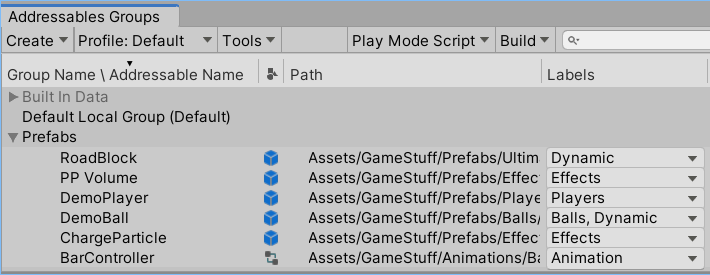
\includegraphics[width=.45\textwidth]{images/addressables.png}}
  \caption{使用Addressables}
  \label{fig:addressables}
\end{figure}

\subsubsection{创建}
\quad

场景物体在创建时往往不止于把Prefab置入场景中,还需要一定程度的初始化。本项目存在服务端、客户端一体的特殊性,同一场景物体在服务端和客户端虽然Prefab一致,但可能需要通过不同的初始化流程,使其特化出不同的性质。例如,作为球类物理游戏,赛场上的球在服务端需要添加刚体,使其具有物理性质,还要附加InfoSender来同步客户端中球的运动;相对的,在客户端的球便无需这些额外的组件。这种差异化的初始化对于程序来说十分重要,保证它在作为服务端或客户端时都正常运行。

对于不同种类的物体,初始化的过程及需要的参数也不尽相同。创建动态物体时可能需要为之附加InfoSender,并提供SendFlag等相关参数;而创建静态物体时基本不会需要这样的操作。这种初始化的多样性导致传输物体创建信息的数据包,格式不太好设计。

本次实践中,使用一组Builder类和一组BuildInfo类来解决场景物体创建的问题。其中BaseBuilder类为抽象泛型类,其一系列子类能够为不同类型的场景物体(如玩家、球、球门等)提供不同的构建逻辑,且能根据BuildType参数来决定执行服务端或客户端的初始化逻辑。创建及初始化所需的参数记录在BaseBuildInfo及其子类中。每个Builder类同一个BuildInfo类对应,在创建物体时需要传入相应类型的BuildInfo对象。例如,球需要使用RigidBuilder传入RigidBuildInfo对象完成创建。所有BuildInfo类都是可序列化的,使用BinaryFormatter可将其对象转换为比特流,进而得以装入数据包中传输。由于BuildInfo对象中包含了物体创建及初始化所需的全部信息,故客户端收到服务端发来的数据包,反序列化为BuildInfo对象后,即可根据其构建出与服务端基本一致的场景物体。只传输BuildInfo,而不用告知使用了何种Builder,是因为各种Builder的对象使用了类似“责任链”的逻辑组合在了一起。每次创建物体时,BuildInfo会从Builder链的根节点传入,直到被能够使用该种BuildInfo创建物体的Builder捕获,进而让此Builder完成物体创建。

另外,Builder还提供了通过场景物体生成BuildInfo的方法,传入自己生成过的场景物体,可根据它们的现状得到对应的BuildInfo。这个方法主要用于服务器向新加入的客户端同步当前已存在的场景物体,让新加入的客户端拥有和服务端大体一致的场景状态。
\subsubsection{销毁}
\quad

相比创建场景物体,销毁它们则十分简单。只需将其通过StageManager移出当前场景物体,并销毁之即可。同样的操作,只要服务端通知,客户端也可以实现同步。

至此,程序中创建、销毁各种场景物体的操作均可由统一的方法作入口执行,并能在服务端与客户端间同步。

\subsection{玩家角色}
\begin{figure}[htbp]
  \centerline{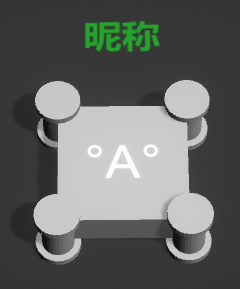
\includegraphics[width=.15\textwidth]{images/player.png}}
  \caption{玩家角色}
  \label{fig:player}
\end{figure}
\subsubsection{移动}
\quad

和大部分俯视游戏不同,游戏角色的移动并非是依据屏幕坐标的,而是为了做到灵活的 $360^\circ$旋转,由前进/后退与旋转两部分组成,键盘上的W/S键用来控制前进后退,鼠标则控制旋转,角度通过屏幕上角色坐标与鼠标坐标所成角度计算。

在综合权衡游戏体验、场地大小、玩家操作等因素后,我们决定将主相机的显示范围设定在以玩家为中心的一块区域而不是整个场地,所以相机也必须跟随着玩家,将玩家置于整个画面的中心,而当玩家处于场地边缘等极端条件下,相机也会做适当的调整,不再移动。

客户端的玩家角色额外拥有InputSender单例脚本,负责记录玩家的输入信息,即玩家都按下了哪些键,玩家的鼠标位置。客户端得到输入信息后不进行处理,而是将其发往服务端,传递至对应的玩家角色,由其特有的PlayerController脚本处理,很好的杜绝了玩家在本地修改内存而进行作弊的可能性。

\subsubsection{能量棒}
\quad

审视玩家角色,会发现它主要由几部分组成——几何体、能量棒、颜文字表情和玩家昵称。除去无实体的表情和昵称,实际上玩家只是一个在尖角嵌入了能量棒的几何体而已。

能量棒如其名,在设定上是充满能量的棒状几何体,体现在游戏中,便是在触碰到物体时会尝试向其释放能量,即施加力。例如,能量棒撞到球会将球弹走;两个玩家的能量棒相撞会导致双方均被击退。在客户端,能量棒触碰物体时会有伸缩的动画效果作为反馈。

为何要有能量棒这种设定?这源于项目规划阶段,感到单纯的几何体依靠碰撞踢球会比较枯燥,游戏要素、操作过于单一,且拥有不同形状几何体的角色似乎并不会受自身形状的影响而产生很大的区别(虽然目前的Demo因时间所限只完成了一种可用角色,但规划时认为最终游戏会有多种角色)。能量棒的出现一定程度上丰富了游戏性。区别于直接使用几何体撞球,目前的游戏中,几何体碰到球后并不会让球一下子弹出,而是能在一定程度上让球随之一同移动,形成带球的效果。想要让球快速射出,使用能量棒便成了较好的选择。让能量棒嵌在几何体的角上,不仅不会影响其大体形状,还使得不同几何体间区分度增加——根据几何体形状不同,尖角数量、分布会产生区别,进而影响能量棒的数量和分布。看似不同几何体角色拥有不同数量的能量棒会让游戏产生平衡性问题,实则可以尝试通过调整角色的其他属性(如速度、转身速度、能量棒力量、大招等)来进行平衡。

能量棒位于几何体的斜角,想用它触球便要旋转角色,直观感觉不是很方便。因为分布在几何体四周的能量棒能粗略地勾勒出其轮廓,以此为灵感,又为能量棒加入了“旋转”机能。旋转能量棒过程中,每个能量棒逆时针移动至前一个能量棒所在位置,整体上所有能量棒可以大致扫过几何体的外围。这个看似没什么用的功能实际上赋予了玩家正面“踢球”的能力,通过旋转能量棒使其在几何体正前方附近碰到球并将之弹出,这样便可以在不旋转角色的同时完成射击。玩家可以点击鼠标左键来旋转能量棒。

实际上,能量棒碰撞物体时施加力的逻辑只在服务端执行,而播放动画效果的逻辑只在客户端执行。这是通过在BallScripts.Servers和BallScripts.Clients引入不同的BarCollision脚本实现的,在能量棒初始化时会根据其所在端挂载相应的脚本。
\subsubsection{必杀技、蓄力}
\quad

必杀技的加入让游戏显得更加刺激,为胜负引入新的悬念。既然是必杀技,那理应是一个不算太差的技能,且很可能效果并非瞬时,而是持续的。设定中,不同种类的角色将拥有不同必杀技,这意味着虽然释放必杀技的操作相同,但释放后执行的逻辑应该是可变的。为了实现可更换、有持续效果的必杀技,定义BaseUltimate抽象类,嵌入服务端的PlayerController中,在必杀技释放时,会调用类中的Update等方法(也可以依靠协程处理必杀技逻辑)。实际特定角色的必杀技,由BaseUltimate的子类实现。当前角色(正方形)的必杀技便是由UltimateCube实现的,会向四周释放逐渐变大的方形几何体。玩家可以点击鼠标中键来释放必杀技。

必杀技如果能随时释放,想必会有损“必杀”之名,也会让赛场变得十分混乱。为此,引入蓄力机制来加以限制。玩家使用鼠标右键或空格键进行蓄力。通过PlayerCharge脚本控制,蓄力时客户端会出现粒子效果,能量棒会充当蓄力条,经由shader处理自底向上逐渐由白变黄,标示蓄力的进度。当蓄力值达到最大时,能量棒的黄色会被发光的金色取代,说明必杀技准备就绪,可以释放。在蓄力时,服务端也会限制玩家的最大速度在较低值,使得蓄力时无法快速移动。

关于能量棒、蓄力、必杀技的示例,见后文图~\ref{fig:result2}。

\subsubsection{队伍、球门、得分}
\quad

队伍、球门、得分,理论上属于游戏机制,却也同玩家有一定联系。

队伍由Team类进行抽象,通过TeamManager管理。设定上,每个场景存在队伍数量上限,且持有若干队伍预设(包含队名、颜色等信息)。玩家连入服务端后,若队伍数尚未达到上限,则根据预设加入新的队伍,否则被比较均匀地分配到老队伍中。玩家离开队伍时,若队伍人数降至0,则解散之。由于队伍是比较抽象的存在,并不像场景物体那样肉眼可见地被创建到场景中,故在网络同步方面与基于场景物体的同步不是很贴合。通过让玩家创建时所用的BuildInfo携带队伍信息,代表玩家属于某队(甚至队伍不存在时创建新队),来让队伍系统尽可能融入场景物体同步。玩家离开队伍时,缺少BuildInfo的辅助,则服务端需要额外通知客户端队伍成员的变更。

球门属于场景物体中较为特殊的一类——它们默认置于场景中,而非稍后才被创建出来。这是因为无法规定球门的标准样式,根据场地不同,球门的样子很可能发生变化。然而,为了让程序正常运行,依然规定了球门必须拥有能修改颜色的队伍标识以及进球的判定区域。设定中每个队伍至少拥有一个球门,且哪个队伍拥有哪些球门是随机的。虽然球门不用被创建到场景中,但它仍然拥有自己的Builder,主要负责根据BuildInfo做初始化,例如同指定队伍绑定。与队伍绑定后,队伍的颜色即是球门队伍标识的颜色。球门的进球判定在服务端通过GoalCollision脚本实现。当球进入球门的进球判定区域时,如果球门拥有队伍,则根据导致进球的玩家来决定得分——其他队玩家进球,为该队加分;己方玩家进乌龙球,为本队扣分(最低为0分)。

至于队伍的得分,由于没有专门针对其的同步机制,故定义为队伍中所有玩家的得分和。每个玩家携带自身的得分信息,以此将得分的同步纳入场景物体的同步机制。每次产生得分,同时更新进球玩家的得分和队伍的总得分,藉由服务器通知客户端,将各端间的队伍比分同步。

\subsection{游戏效果}
\subsubsection{玩家名字}
\quad

当前游戏中的UI并不多,而且也几乎没有需要用到统一管理的操作,所以我们没有编写全局的UI Manager,而是两个场景各有一个专门管理UI的脚本。在连接到服务器之前,玩家需要输入一个自己的昵称,这个名字会在后面的游戏场地上以TextMesh的形式作为玩家的子物体存在,跟随玩家。其中涉及到的变量名跨场景传递是由GameManager实现的。

\subsubsection{小地图}
\quad

小地图是由一个专门的小地图摄像机和材质实现的,让摄像机把拍摄到的东西渲染到材质上,再将材质赋给Raw Image,即可在Canvas上显示小地图。为了让玩家能够清晰地从小地图中获得足球位置,我们还给小地图摄像机添加了一个边缘检测的shader,做出类似描边的效果。

\begin{figure}[htbp]
  \centerline{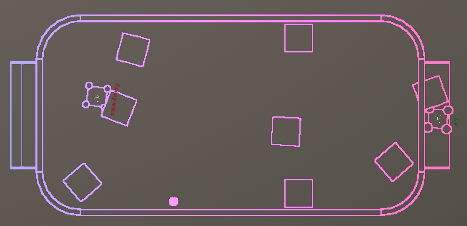
\includegraphics[width=.38\textwidth]{images/mini-map.png}}
  \caption{小地图}
  \label{fig:minimap}
\end{figure}

\subsubsection{后期处理}
\quad

我们用Unity的PostProcessing插件为游戏添加了丰富的后期处理效果,其中有增强画面美观度的暗角,增强画面表现力的辉光,增加画面真实感的动态模糊和增加用户反馈的色彩分离。色彩分离效果的强度是由代码控制的,这样我们会在能量棒发生碰撞时调用相关方法,一旦碰撞,整个画面都会出现色彩分离。

\begin{figure}[htbp]
  \centerline{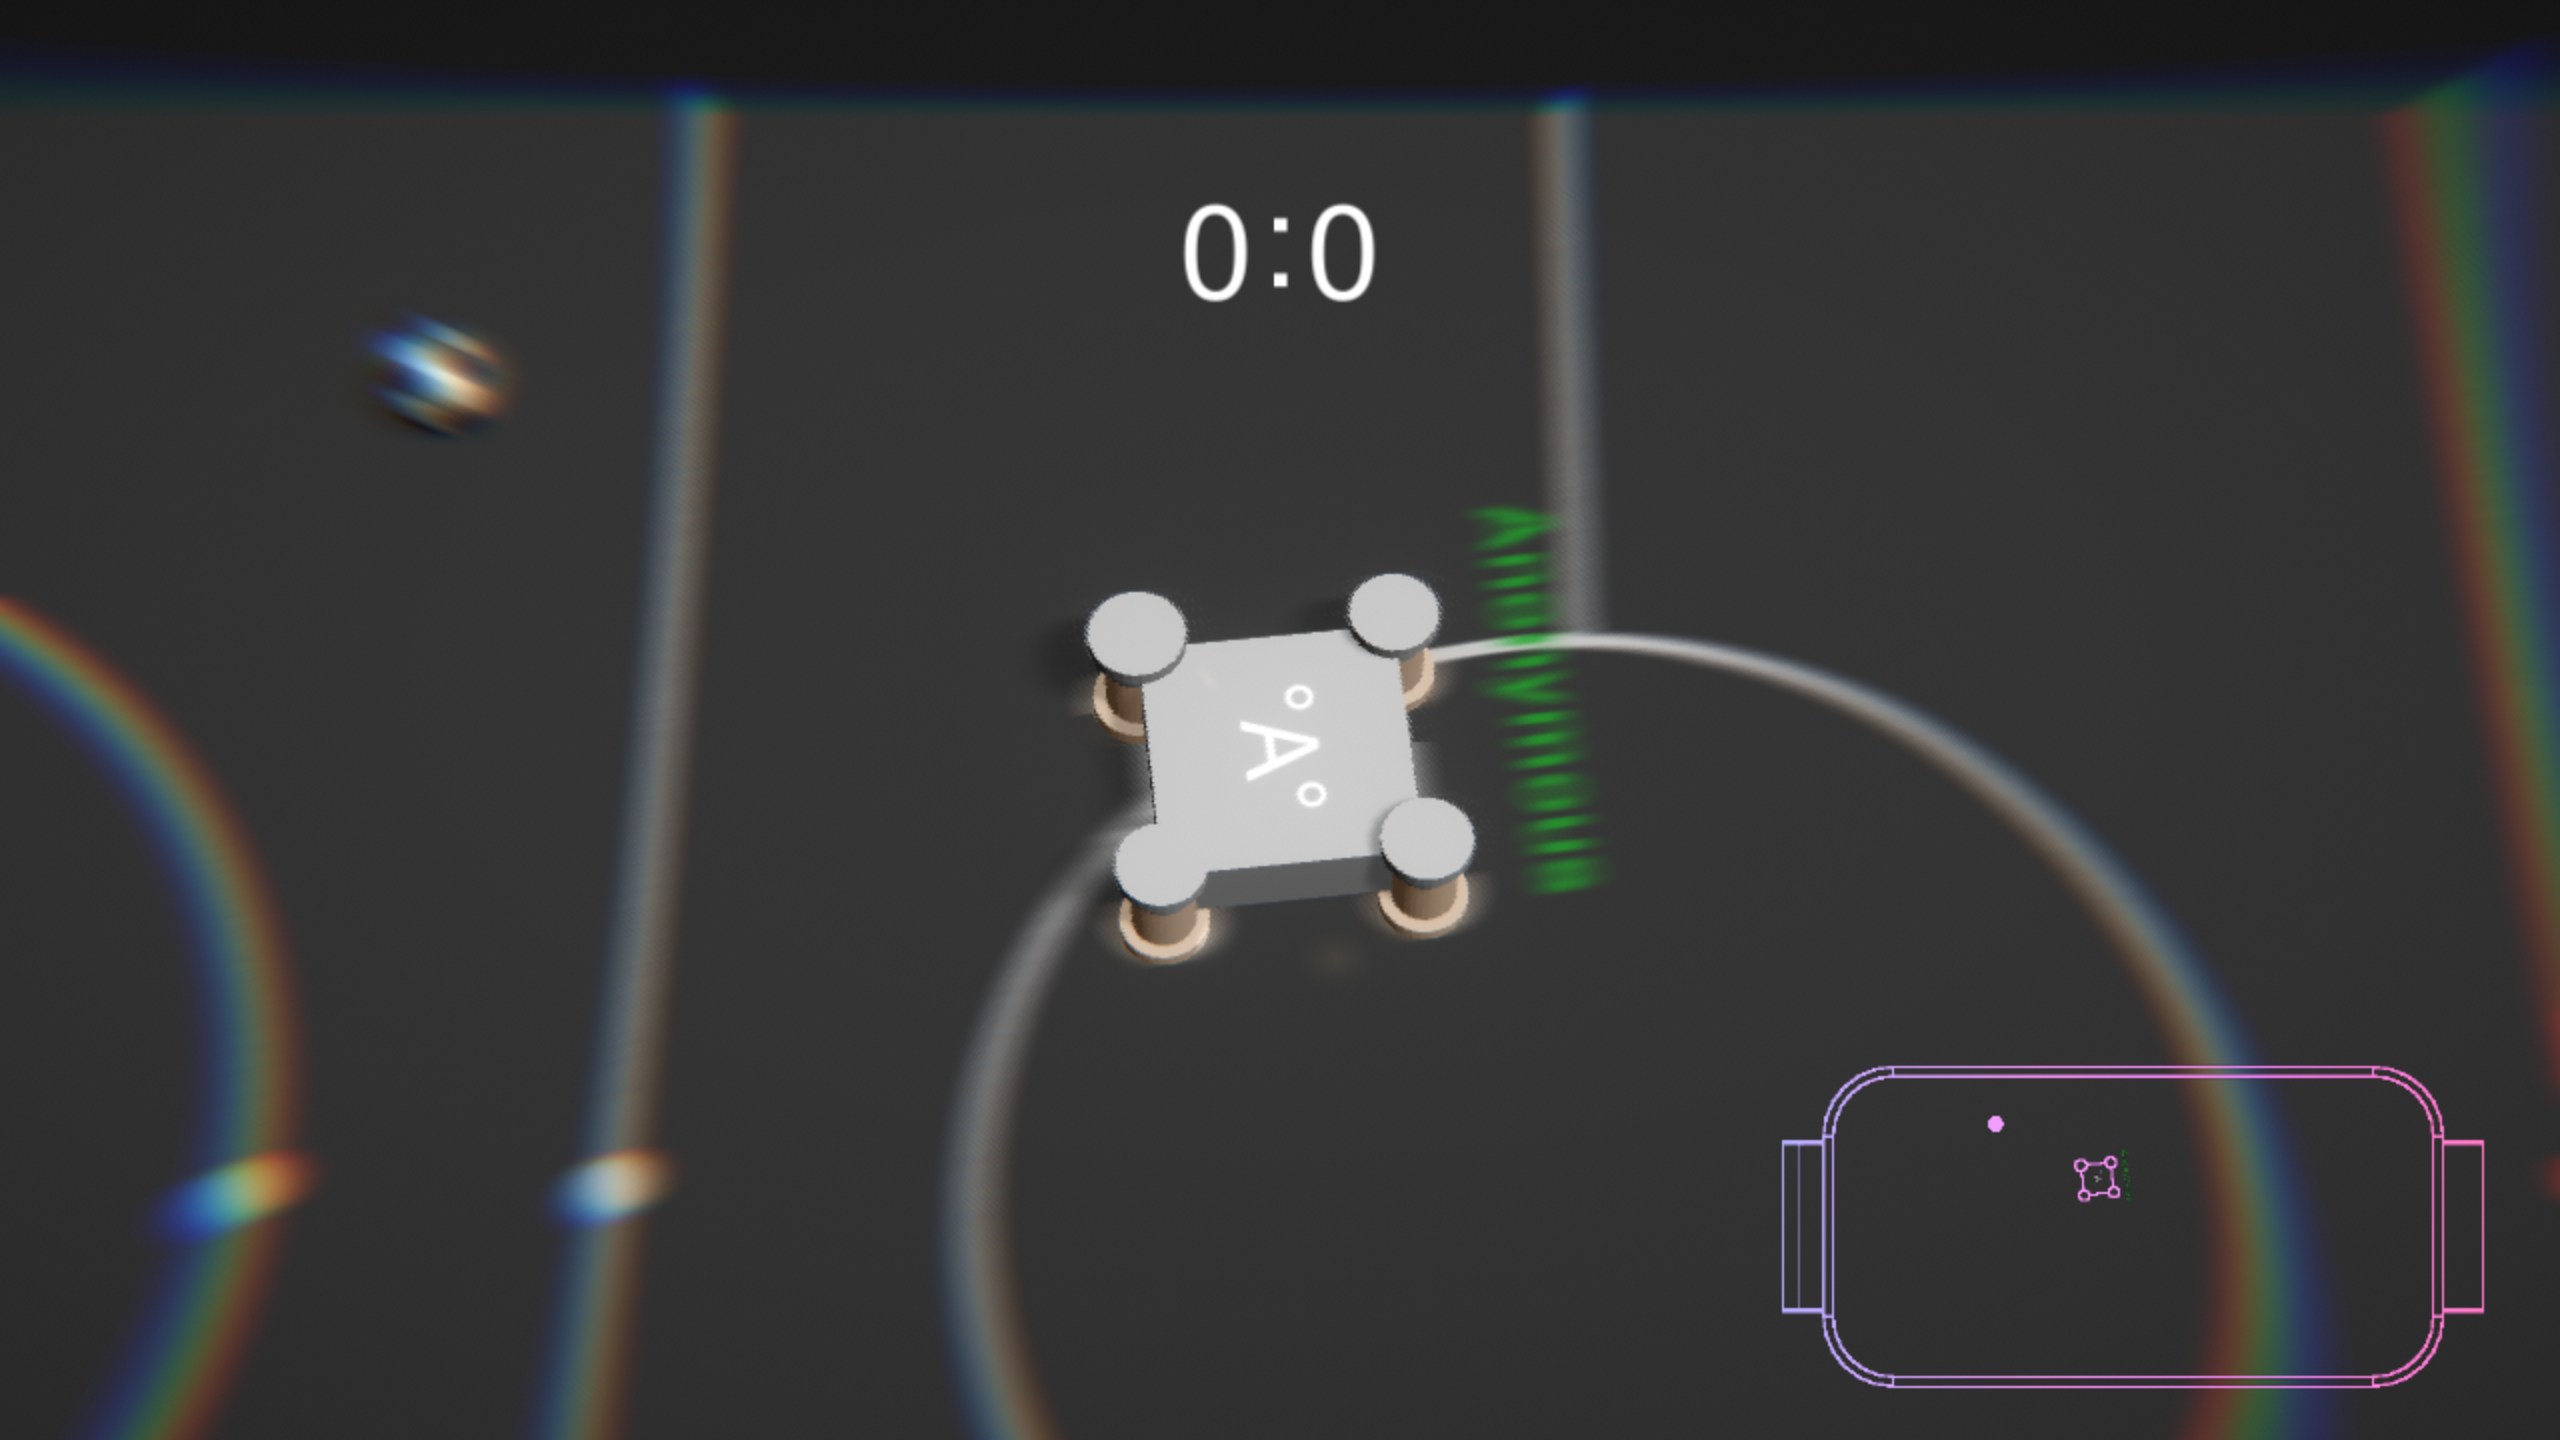
\includegraphics[width=.38\textwidth]{images/pp.png}}
  \caption{后期处理效果}
  \label{fig:pp}
\end{figure}

\subsection{实用代码}
\subsubsection{单例基类}
\quad

程序中使用了许多单例,这种模式使得一个类能拥有唯一的对象,且该对象能够被全局访问,使用其编写一些游戏系统、管理相关的逻辑会比较方便。

对于各种单例类,用来使之表现出单例性质的逻辑是共通的,故可将其提炼出来进行复用\cite{myCite:singleton}。通过把一个Singleton泛型类作为基类,实现了将任意MonoBehaviour的子类作为单例类使用。这种单例类有不跨场景和跨场景两种模式——若脚本实例初始便在场景中存在,则单例使用范围仅限当前场景;若初始不在场景中,则会生成能够跨场景存在的单例。这种单例的实现是线程安全的。

\subsubsection{线程管理}
\quad

Unity中使用多线程的情况较少,在其他线程上UnityEngine相关逻辑很可能无法正常运作。但实际开发测试过程中,发现有时调用一些非MonoBehaviour子类的静态方法,在Unity编辑器中也无法正常执行。根据\cite{myCite:Tom}的做法,引入了ThreadManager来尝试解决这样的问题。该类为MonoBehaviour的子类,对象会跨场景地存在于游戏中,在全局以委托的形式接收各种逻辑,并在FixedUpdate中统一执行。经过这样的封装,使得各种逻辑能够在Unity主线程上运行。处理数据包的逻辑均会经历这样的封装操作。

\subsubsection{网络标识特性}
\quad

程序使用较多的场景物体同步,只涉及到了物体的创建、销毁等,即对物体本身的同步。这种同步是比较粗粒度的,无法做到随时同步物体内部的种种细节(如玩家得分、蓄力状态等)。通过引入特性(Attribute),将需要同步的类和其类成员取名标记,进而可以基于反射完成对类中细节的同步。本项目使用NetworkMarkerAttribute标识可被同步的字段、属性、方法,使用NetworkClassAttribute标识包含这些类成员的类,而NetworkMarkerManager用来管理这些标识。经过如此处理,对于任何场景物体,服务端可以尝试让客户端同步其被标识的字段与属性,或通知客户端调用被标识的方法。玩家角色蓄力值的同步便依靠此机制实现。

\section{实验结果}

\begin{figure}[htbp]
  \centerline{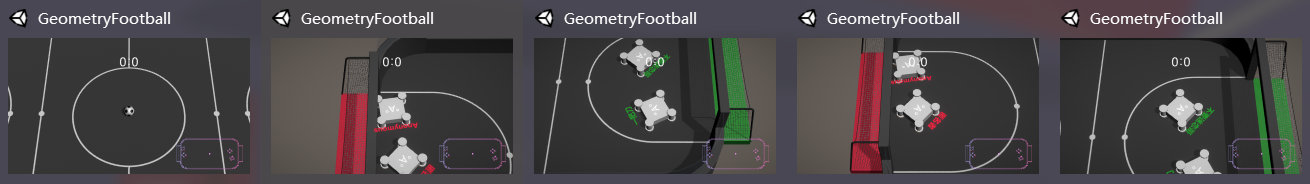
\includegraphics[width=.46\textwidth]{images/result1.png}}
  \caption{在本地开启一个服务端和四个客户端}
  \label{fig:result1}
\end{figure}
  根据图~\ref{fig:result1},每个客户端在加入游戏中都会按照规则分配给相应的队伍。

\begin{figure}[htbp]
  \centerline{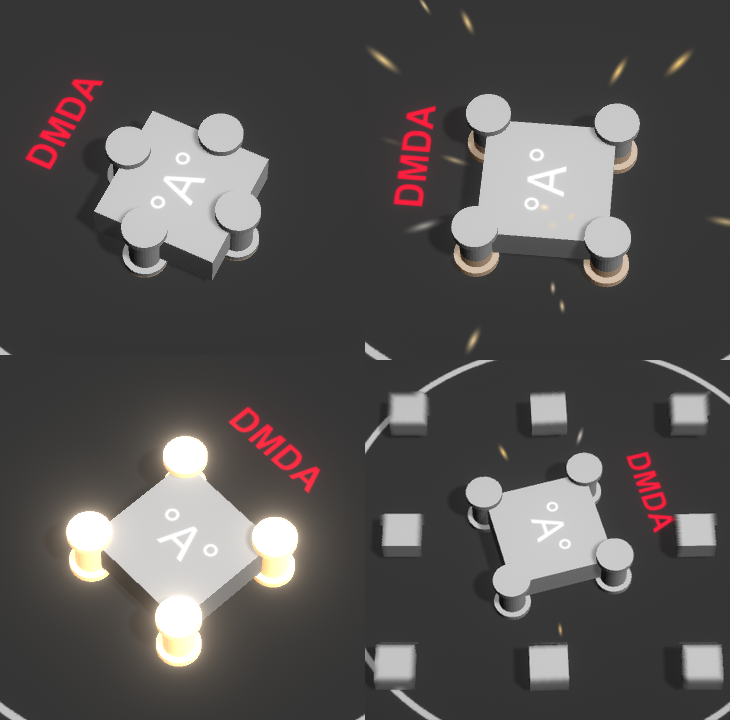
\includegraphics[width=.32\textwidth]{images/result2.png}}
  \caption{动作展示}
  \label{fig:result2}
\end{figure}
  图~\ref{fig:result2}分别展示了:旋转能量棒、蓄力、蓄力完成、释放必杀技。

  在实际测试中,即使客户端和服务端的机器在两个间隔较远的房间,也可以通过校园网分配的IP地址正常进行游戏,甚至还可以借助游侠对战平台等软件构造出的虚拟局域网来进行互联网范围的联机游戏,延迟和帧数还有些差强人意,但对可玩性影响有限。

\section{结论}
在这次项目中,我们开发出了一个完整的可以进行多人在线对战的游戏,它的游戏部分不是仅为联网而做的demo,而是一个真正可玩、充满对抗性、元素丰富的竞技游戏,而它的联网部分在我们的测试中也表现出色,虽然目前尚未有房间系统,但完全可以通过开多个客户端并设定不同端口的方式来达到类似房间系统的效果。联网游戏的开发比单击游戏要复杂很多,许多原先可以轻松实现的效果在联网游戏中都要充分考虑如何创建、同步、销毁,服务端、客户端的代码如何解耦,怎样来减少运行时的开销,在克服重重困难后,小组成员从中汲取了许多经验,颇具收获。

未来,我们可以进一步提升游戏性,加入三角、圆形、五角星等新的拥有不同大招的角色,引入场地道具等系统,甚至可以去做新的场地、多个球门、吃鸡模式;性能方面也有较大优化的空间,当前服务器必须以图形界面运行,如果将其改为纯控制台,或许就可以真正部署到运行 Linux系统的服务器上;至于游戏效果,可以为游戏添加背景音乐及音效,使角色的表情和动画更加生动,丰富UI,乃至让游戏画面看起来更精美。

% \section*{References}

\bibliography{myCite}
\bibliographystyle{IEEEtran}

\end{document}
